\section{from light to electron}
Human have long history of harnessing light and creating optical microscopes that allow us to look closer. The resolution of the microscope is physically limited by the wavelength of the light, as framed by Abbe's diffraction limit:
\begin{equation}
	d = \frac{\lambda}{2\cdot NA}.
\end{equation}
This states that the smallest distance $d$ at which two points can be distinguished as separate is approximately half of the wavelength of light being used, modified by the numerical aperture $NA$ of the objective lens. This means for a visible light of $\lambda \approx 500nm$, the best possible resolution is around $200$ to $250nm$. By developing light sources with shorter wavelength, scientists were able to push the optical boundary. With the development of UV microscopy in the 1920s, the spatial resolution was pushed to approximately $100nm$. 

People start to look for something with shorter wavelength to resolve finer structures. According to the matter wave theory proposed by Louis de Broglie in 1924, matter exhibits wave-like behavior with a wavelength $\lambda$ inversely proportional to its momentum $p$: 
\begin{equation}
	\lambda = \frac{h}{p},
\end{equation}
where $p$ is the Planck constant. 

This inspired people to look into electrons, whose wavelength is orders of magnitude smaller than that of light, and whose momentum is easier to manipulate through electric field. Ernest Ruska made the most important foundational contributions to electron optics and designed the first electron microscope in 1930s. Borrowing the same set up in a conventional microscope, Ruska designed a transmission electron microscope(TEM), by letting the electron beam piercing through a thin section of the object. The invention of TEM brought the resolution to about $10nm$, achieving the best resolution at that time. 

Scanning tunneling microscope(STM) marks another attempt to manipulate electrons for high-resolution imaging. However, it is not a true microscope that gives a direct image of an object; instead, it is more like how a blind person reads the Braille as shown in Figure \ref{fig:braille} panel a). Similar to how fingers detect the impressed characters, \ac{STM} scans a metallic tip to "sense" the structure of a sample surface, as illustrated in pane b). However, the sensing is not down by making mechanical contact, instead, an \ac{STM} tip is placed very closed(\textasciitilde $1nm$) to the sample surface and by applying a bias voltage across the tip-sample junction, electrons from one side will travel through the vacuum barrier to the other side, creating a current. The principle enabled this counter intuitive movement of electron across the vacuum barrier is called quantum tunneling effect, hence the name of the instrument. The first \ac{STM} was introduced by Gred Binnig and Heinrich Rohrer in 1981. Next year in 1982, Binnig and Rohrer performed the first surface topography with this new-born; they inspected the surface of Si(111) and observed the $7 \times 7$ reconstruction as shown in Figure \ref{figure:si111_binnig}\cite{binnig77Reconstruction1983}. This direct observation of the 12 adatoms in a unit cell allows them to propose a modified model for the adatoms. With the invention and development of \ac{STM}, scientists for the first time, were able to visualize and manipulate atomic features with a picometer($10^{-12}$m) resolution.
\begin{figure}
	\centering
	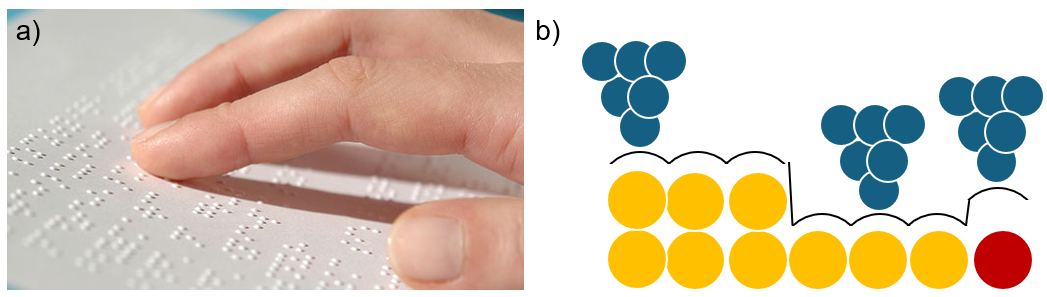
\includegraphics[width=0.8\textwidth]{braille.png}
	\caption{Analogy between the Braille reading and STM topography}
	\label{fig:braille}
\end{figure}
The foundational work done by Ruska, Binnig and Rohrer on electron microscope was awarded the 1986 Nobel Price in Physics. From the earliest optical instruments to the advent of electron-based probes, each leap in resolution has revealed new structural detail. STM represents the culmination of this progression, pushing beyond the limits of conventional electron optics by harnessing quantum tunneling rather than direct imaging. With its ability to map surfaces atom by atom, STM opens up entirely new fields, including the study of point defects in quantum materials

\begin{figure}
	\centering
	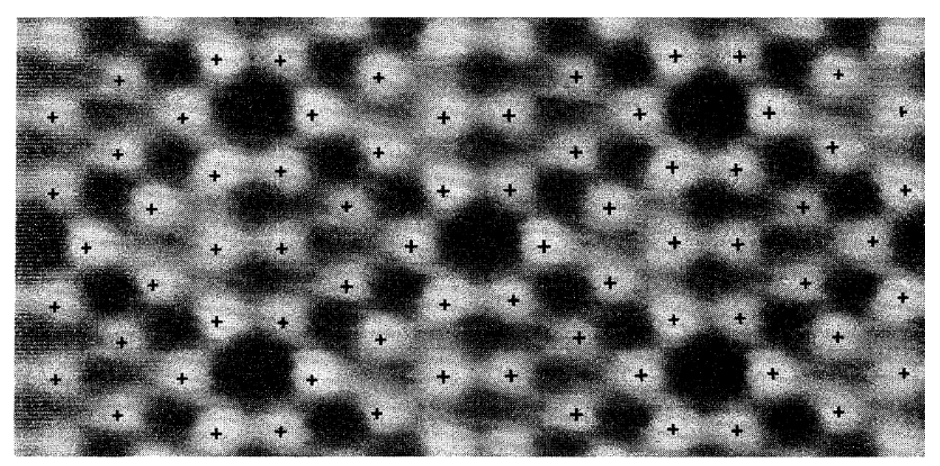
\includegraphics[width=0.8\textwidth]{Si111_binnig.png}
	\caption{}
	\label{figure:si111_binnig}
\end{figure}

In this chapter, we will first explain the theory of \ac{STM}, then introduce the configuration of a modern \ac{STM}, and close with an introduction on the instrument we used for this study. 

\section{Theory of STM}
In essence, an \ac{STM} works by collecting and analyzing the tunneling current between the tip and sample. Thus, the quantitative understanding of the tunneling current is the core of theory of \ac{STM}, and thus the focus of this section. We will first give a overview on the quantum tunneling and the theory development in history, then we will elaborate on the derivation of tunneling current in a typical tip-sample geometry.

\subsection{quantum tunneling and development of STM theory}
Quantum tunneling described the behavior of quantum mechanical object passing through a potential barrier that is higher than their energy. The word passing through is adopting the classical particle point of view, for a quantum mechanical object that exhibit wave-particle duality, we should say that the wave function of this object has a finite amplitude on the other side of the barrier, and thus a non-zero probability density to find the object in the classically prohibited region. Quantitatively, according to the WKB approximation, the transmission probability $T$ for a particle with mass $m$ and energy $E$, given a potential barrier of $V$ with width $\alpha$ is: 
\begin{equation}
	T \approx e^{-\alpha\sqrt{\frac{8m}{\hslash^2}(V-E)}}. 
\end{equation}
In fact, according to de Broglie's  matter wave theory, even a classical object could theoretically tunnel through a seemly forbidden barrier, just extremely unlikely: the probability for a baseball traveling at 40 m/s to tunnel through a 10 cm thick brick wall is approximately $e^{-10^{33}}$. 

The development of theory of quantum tunneling can be dated in 1928, when Robert Oppenheimer developed a time-dependent perturbation method trying to explain the ionization of hydrogen in an apply field\cite{oppenheimerThreeNotesQuantum1928}. A more general theory for a metal-insulator-metal junction is introduced by Bardeen in 1961\cite{bardeenTunnellingManyParticlePoint1961}, 20 years before the birth of \ac{STM}. Two years after the invention of \ac{STM}, Tersoff and Hamann extended Bardeen's theory to model an ideal STM tip-sample junction, which successfully interpreted the topography of Au crystal \cite{tersoffTheoryApplicationScanning1983}\cite{tersoffTheoryScanningTunneling1985}. Later, Lang found that one can effectively model the \ac{STM} operation with tunneling between only the single atom on the end of a tip(the acting atom) and the single atom on the surface, revealing the atomic nature of the \ac{STM} \cite{langVacuumTunnelingCurrent1985}\cite{langSpectroscopySingleAtoms1986}\cite{langApparentSizeAtom1987}. Inspired by the atomic picture, Julian Chen built a three-dimensional model of the tunneling considering different tip configurations by expanding the asymptotic wave function of the acting atom\cite{chenTunnelingMatrixElements1990}\cite{chenTheoryScanningTunneling1988}. 

Since our work include using a simple tungsten tip and a low bias voltage(amplitude within 1V), it is sufficient to use the result from Teroff and Hamann.  

\subsection{Tunneling current}
According to Fermi's golden rule, the transmission probability between the tip and sample is directly related to the matrix element $M_{ts}$ between the tip's state $\psi_{t}$, sample's state $\psi_{s}$, and their corresponding electron density $\rho$. When applied a small bias voltage $V_s$ to the sample, we can write:
\begin{align}
	P_{t->s} &= \frac{2\pi}{\hslash}\int_{-\infty}^{\infty}|M_{ts}|^2\rho_s(\epsilon + eV_s)[1-f(\epsilon+eV_s)]\cdot \rho_t(\epsilon)f(\epsilon) d\epsilon \\
	P_{s->t} &= \frac{2\pi}{\hslash}\int_{-\infty}^{\infty}|M_{ts}|^2\rho_s(\epsilon + eV_s)f(\epsilon+eV_s)\cdot \rho_t(\epsilon)[1-f(\epsilon)] d\epsilon,
\end{align} 
where $f$ represents the Fermi-Dirac function. It is worth noting that in order to use Fermi's golden rule, an equilibrium condition is assumed; this is generally satisfied as the internal relaxation time scale for metallic electrodes are in the range of femtosecond to picosecond, which is much smaller than milliseconds settling time used in standard \ac{STM} measurements. 

The tunneling current proportional to the net transmission probability across tip and sample, under one key assumption: the tunneling must not change the occupation number of both the sample and tip side. This is generally true since the tunneling current is normally is the order of nano-Ampere to pico-Ampere; this correspond to approximately $10^6 \textasciitilde 10^9$ electrons per second, which is tiny compared to the total number of electrons in both electrodes. Thus we can write the tunneling current $I_t$:
\begin{align}
	I_t & = 2e(P_{t->s}-P_{s->t})\\
	& = 2e \cdot \frac{2\pi}{\hslash}\int_{-\infty}^{\infty}|M_{ts}|^2\rho_t(\epsilon) \rho_s(\epsilon + eV_s) \cdot[f(\epsilon) - f(\epsilon + eV_s)] d\epsilon.
\end{align}
The factor of 2 is a result of the spin degeneracy. At low temperature, when $k_BT<<V_s$, we can replace the Fermi-Dirac distribution function $f$ with a step-wise function, and simplifies the integral to: 
\begin{equation}
	\label{eq:I_t}
	I_t = \frac{4e\pi}{\hslash}\int_{0}^{eV_s}|M_{ts}|^2\rho_t(\epsilon - eV_s) \cdot \rho_s(\epsilon)d\epsilon. 
\end{equation} 
From Equation \ref{eq:I_t}, we note that the tunneling current is proportional to both $\rho_t$ and $\rho_s$, since we are interested in probing the sample, we can simply pick the tip to have a featureless $\rho_t$. This can be achieved by using simple metal and their alloys; typically, \ac{STM}s today use tips made of tungsten or a platinum-iridium.


\vspace{1em}
\noindent\textbf{Approximating the matrix elements}

\noindent In a semiclassical picture with WKB approximation, by estimating the transmission probability through a square barrier of height $W = (W_t + W_s)/2$, where $W_t$ and $W_s$ are the work function for the tip and sample respectively, we can get the matrix element $M_{ts}$: 
\begin{equation}
	|M_{ts}|^2 = e^{-2\kappa d},
\end{equation}
where $\kappa = \sqrt{2mW}/\hslash$.

However, the quantum mechanical determination of the matrix element is much more complex. Intuitively, it can be pictured as the overlapping of sample wave function and tip wave function within the insulating barrier. Here, I will follow the historical development to show how the matrix element is determined. Bardeen first made a significant leap by formulating a general expression for a metal–insulator–metal junction under a few key assumptions. Later, Tersoff and Hamann applied this framework to the idealized STM setup, featuring a sharp tip facing a flat sample surface.

"The way to derive Bardeen's tunneling theory is not straightforward; it does not proceed by routine application of textbook techniques"\cite{gottliebBardeensTunnelingTheory}; this lead to many direct usage of his work without proper explanation on its provenance. Here I follow the approach of C.B.Duke\cite{dukeTunnelingSolids1973}. If the readers are curious, a very comprehensive and accessible tutorial can be found here\cite{gottliebBardeensTunnelingTheory}. 

To start, we can first write the general expression of matrix element in real space as: 
\begin{equation}
	\label{eq:bardeen_1}
	\braket{\phi_{\mu}|H-H_s|\psi_{\nu}} = \int(V(\mathbf{r})- V_s(\mathbf{r})\phi_{\mu}(\mathbf{r})*\psi_{\nu}(\mathbf{r}))dr,
\end{equation}

where $\phi_{\mu}$ and $\psi_{\nu}$ are the eigenstates of the tip Hamiltonian $H_t$ and sample Hamiltonian $H_s$, respectively. That is $H_t \phi_{\mu} = \epsilon_{\mu} \phi_{\mu}$, and $H_s \psi_{\nu} = E_{\nu} \psi_{\nu}$. Note that this is a key assumption in Bardeen's formalism, that the junction is in the weak tunneling condition, ie, the sample potential($V_s$) and the tip potential $V_t$ does not penetrate into each other. 

Bardeen then artificially separate the barrier region into two part by drawing a "separation surface" $\mathbf{S}$; the volume that is close to the tip side is denoted as $\mathbf{T}$, and $\mathbf{S} = \partial \mathbf{T}$.

We can then observe that the total Hamiltonian $H$ equate $H_t$ in region $\mathbf{T}$ due to the absence of sample potential $V_s$: 
\begin{equation}
	\label{eq:bardeen_2}
	\begin{aligned}
		0 &= \braket{\psi_{\nu}|(H-H_t)|\phi_{\mu}^*}_{\mathbf{T}}\\
		 &= \int_{T} \psi_{\nu}(\mathbf{r}) \left( H - H_{t} \right) \phi_{\mu}^*(\mathbf{r}) \, d\mathbf{r} 
		= \int_{T} \psi_{\nu}(\mathbf{r}) H \phi_{\mu}^*(\mathbf{r}) \, d\mathbf{r} 
		- E_{\nu} \int_{T} \psi_{\nu}(\mathbf{r}) \phi_{\mu}^*(\mathbf{r}) \, d\mathbf{r} \\
		&= -\frac{\hslash^2}{2m} \int_{T} \psi_{\nu}(\mathbf{r}) \Delta \phi_{\mu}^*(\mathbf{r}) \, d\mathbf{r} 
		+ \int_{T} \psi_{\nu}(\mathbf{r}) V(\mathbf{r}) \phi_{\mu}^*(\mathbf{r}) \, d\mathbf{r} 
		- E_{\nu} \int_{T} \psi_{\nu}(\mathbf{r}) \phi_{\mu}^*(\mathbf{r}) \, d\mathbf{r}.
	\end{aligned}
\end{equation}

And similarly, $H - H_s$ is a zero operator in the barrier region that is not $\mathbf{T}$. Thus the integral in Equation \ref{eq:bardeen_1} can be reduced to region $\mathbf{T}$:   
\begin{equation}
	\label{eq:bardeen_3}
	\begin{aligned}
		&\langle \phi_{\mu} | H - H_{\text{s}} | \psi_{\nu} \rangle \\
		&= \int_{T} \phi_{\mu}^*(\mathbf{r}) \left( H - H_{\text{sam}} \right) \psi_{\nu}(\mathbf{r}) \, d\mathbf{r} 
		= \int_{T} \phi_{\mu}^*(\mathbf{r}) H \psi_{\nu}(\mathbf{r}) \, d\mathbf{r} 
		- \epsilon_{\mu} \int_{T} \phi_{\mu}^*(\mathbf{r}) \psi_{\nu}(\mathbf{r}) \, d\mathbf{r} \\
		&= -\frac{\hslash^2}{2m} \int_{T} \phi_{\mu}^*(\mathbf{r}) \Delta \psi_{\nu}(\mathbf{r}) \, d\mathbf{r} 
		+ \int_{T} \phi_{\mu}^*(\mathbf{r}) V(\mathbf{r}) \psi_{\nu}(\mathbf{r}) \, d\mathbf{r} 
		- \epsilon_{\mu} \int_{T} \phi_{\mu}^*(\mathbf{r}) \psi_{\nu}(\mathbf{r}) \, d\mathbf{r}.
	\end{aligned}
\end{equation}

Subtracting Equation \ref{eq:bardeen_2} from Equation \ref{eq:bardeen_3}, we get: 
\begin{equation}
	\label{eq:bardeen_matrixelement}
	\begin{aligned}
		\braket{\phi_{\mu}|H-H_s|\psi_{\nu}} &= \int_\mathbf{T}\phi_{\mu}^*(\mathbf{r})(-\frac{\hslash^2}{2m} \nabla \psi_{\nu}(\mathbf{r}) - \epsilon_{\mu}\psi_{\nu}(\mathbf{r}))dr \\ 
		& - \int_\mathbf{T}\psi_{\nu}(\mathbf{r})(-\frac{\hslash^2}{2m} \nabla \phi_{\mu}^*(\mathbf{r}) - E_{\nu}\phi_{\mu}^*(\mathbf{r}))dr.
	\end{aligned}
\end{equation}
By considering only $\epsilon_n \approx E_j$, we can get:
\begin{align}
	\label{eq:bardeen4}
	\braket{\phi_{\mu}|H-H_s|\psi_{\nu}} &\approx -\frac{\hslash^2}{2m}\int_\mathbf{T}\nabla \cdot [\phi_{\mu}^*(\mathbf{r})\nabla\psi_{\nu}(\mathbf{r})-\psi_{\nu}(\mathbf{r})\nabla\phi_{\mu}^*(\mathbf{r})]dr\\ \label{eq:bardeen5}
	& = -\frac{\hslash^2}{2m}\int_{\partial\mathbf{T}}[\phi_{\mu}^*(\mathbf{r})\nabla\psi_{\nu}(\mathbf{r})-\psi_{\nu}(\mathbf{r})\nabla\phi_{\mu}^*(\mathbf{r})]\cdot d\mathbf{n}.
\end{align}

This results in Bardeen's approximation of the matrix element, where $\mathbf{n}$ represent the normal vector of $\partial\mathbf{T}$, pointing away from the tip region.  

Tersoff and Hamann took Equation \ref{eq:bardeen5} and applied it \ac{STM}. They considered the sample being a periodic crystal, with the sample states following a Bloch wave in x-y plane. The states are weighted by an exponentially decreasing decay factor and the sample wave function $\psi_{\nu}(r)$ can be expressed as:
\begin{equation}
	\label{eq:sample_wavefunction}
	\psi_{\nu}(r) = \sum_G C_{k_{||},G} e^{-\alpha_{\nu,G}\cdot z }e^{i(k_{||}+G)x},
\end{equation}
where $K_{||}$ is the component of wave vector that is parallel to the surface. $G$ is the in-plane reciprocal lattice wave vector. And $\alpha_{n,G} = \sqrt{|k_{||}+G|^2 + \kappa_{\nu}^2}$, where $\kappa_{\nu} = \sqrt{2m(W_s - E_{\nu})/\hslash^2}$ and $W_s$ is the work function of sample. 

The tip end was assumed to be locally spherical with a radius of R centered at tip center $\mathbf{r_0}$. The tip wave function outside of the tip region can be modeled as:
\begin{equation}
	\label{eq:tip_wavefunction}
	\phi_{\mu}(r) = A_{\mu} \frac{e^{-\kappa_{\mu} |\mathbf{r-r_0}|}}{|\mathbf{r-r_0}|},
\end{equation}
With $\kappa_{\mu} = \sqrt{2m(W_t-\epsilon_{\mu})/\hslash^2}$. A schematic of the set up is shown in Figure.\ref{fig:tersoff}. 
\begin{figure}
	\centering
	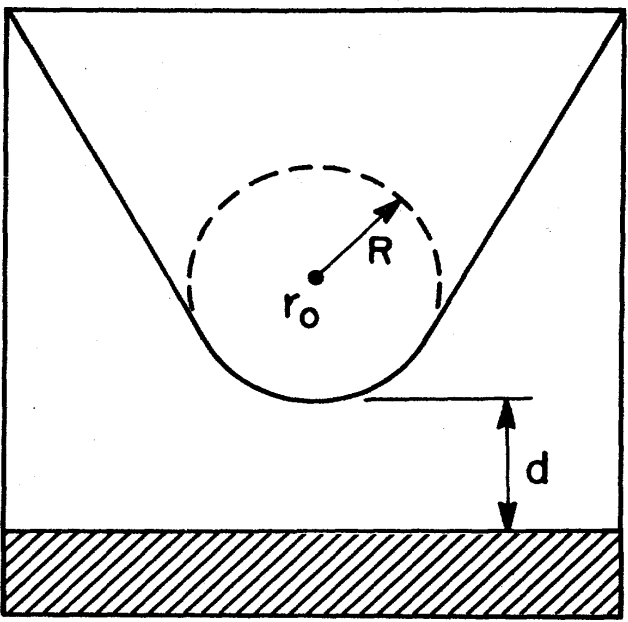
\includegraphics[width=0.8\textwidth]{tersoff_geometry.png}
	\caption{A schematic of the set up used by Tersoff and Hamann. figure adopted from reference \cite{tersoffTheoryScanningTunneling1985}}
	\label{fig:tersoff}
\end{figure}

They then plug Equation \ref{eq:sample_wavefunction} and \ref{eq:tip_wavefunction} into Equation \ref{eq:bardeen5}, and get the matrix element: 
\begin{equation}
	\label{eq:matrixelement_final}
	M_{\mu \nu} = -\frac{2\pi\hslash^2}{m}A_{\mu}\psi_{\nu}(\mathbf{r_0})
\end{equation}

The final expression for matrix element is proportional to the sample's surface wave function at the center of the tip. This is the fundamental reason why \ac{STM} is considered a local probe. Moreover, $A_{\mu}$ contains the exponential decay term; the decay length is often sub-angstrom, allowing extremely fine control of the tip-sample junction distance. 

We now recall that in the weak tunneling limit, the low-temperature net tunneling current is given by Equation \ref{eq:I_t}:
\begin{equation}
	I = \frac{4\pi e}{\hslash} \int_0^{eV}|M_{\mu \nu}|^2 \rho_t(\epsilon - eV) \cdot \rho_s(\epsilon) d\epsilon.
\end{equation}
we plug in the matrix element \ref{eq:matrixelement_final} and get:
\begin{equation}
	I(V) \propto \int_0^{eV}  \rho_s(\mathbf{r_0},\epsilon) \rho_t(\epsilon-eV) d\epsilon,
\end{equation}
where $\rho_s(\mathbf{r_0},\epsilon) = \sum_{\nu} |\psi_{\nu}(\mathbf{r_0})|^2 \delta(\epsilon - E_{\nu})$, is the local density of state(LDOS) of the sample at the tip center. We then substitute $E = E_F+ \epsilon - eV$. And at the low bias regime, the electron density of tip near the Fermi level can be seen as constant, we thus have: 
\begin{equation}
	I(V) \propto \int_{E_F}^{E_F+ eV}  \rho_s(\mathbf{r_0},E) dE,
\end{equation}

We can further take the derivative of the current with respect to the voltage, and get: 
\begin{equation}
	dI/dV \propto \rho_s(\mathbf{r_0},E_F + eV),
\end{equation}
which setting the theoretical foundation for Scanning Tunneling Spectroscopy(STS) measurement. 

\section{Configuration of an STM}
There are four components of a typical STM, they are tip-sample junction, the motion control system, feedback loop $\&$ controller, and environment control system. 

The tunneling tip-sample junction is the most important components, it is made of a metallic tip and a conductive flat sample. Tips are normally made of Tungsten and Platinum-Iridium wires. Electrical etching or mechanical cutting can yield apexes that are sharp under the optical microscope. Due to the atomic nature of \ac{STM} measurements, an atomically sharp tip is desired; while it is hard to obtain, tip-processing procedures like Ar-sputtering or electron annealing can generally help the tip condition. Conductive samples are normally prepared in Ultra High Vacuum(UHV) environment with pressure below $10^-9 mbar$ to prevent contamination from other molecules. The sample is mounted on a sample stage that allows relative position with respect to the tip. 

The motion of STM tip is driven by a set of piezoelectric scanners. Piezoelectricity is the ability of certain materials to generate a electric potential when a mechanical stress is applied. Inversely, when an electric field is applied, piezoelectric material causes mechanical deformation. A typical piezoelectric material used in STM is Quartz, which exhibits a high piezoelectric sensitivity. With typical displacement coefficients on the order of a few picometers per volt, sub-angstrom control of the STM tip position is allowed using modest driving voltages. Moreover, quartz also has rigid mechanical property and low thermal expansion, which are essential for durable operations across a wide temperature range.
 \begin{figure}
 	\centering
 	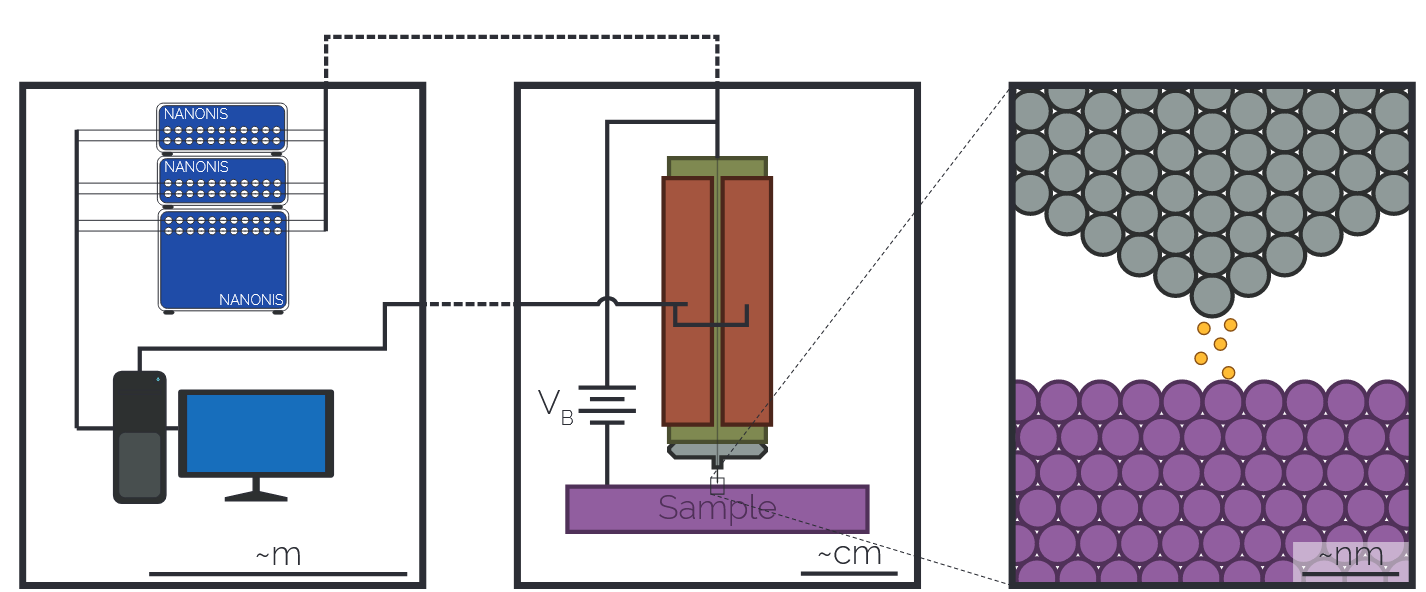
\includegraphics[width=0.8\textwidth]{STM_schematic.png}
 	\caption{Schematic of a typical STM setup. Right: The tip–sample tunneling junction, consisting of a metallic tip (commonly W or Pt–Ir) brought within atomic distance of a clean, conductive sample surface prepared under UHV conditions. Middle: The STM head, roughly the size of a human fist, contains the piezoelectric scanner that provides sub-angstrom control of the tip motion. Left: Control electronics, including the bias source, current amplifier, and PID feedback circuit, regulate the tunneling current and tip–sample distance during operation. Together with vibration isolation, cooling, and vacuum systems, these components form the complete STM instrument.}
 	\label{fig:stm_schematics}
 \end{figure}
 
A set of controllers is used to apply bias voltage, monitor the tunneling current and manipulate the motion of the tip. A DC bias voltage is applied across the tip and sample, the experimental setup in this thesis applied the bias voltage to the sample while grounding the tip. Feedback electronics with a proportional-integral-derivative(PID) feedback mechanism are employed to keep the tunneling current stable during scanning. If the current falls, the tip is driven closer to the surface; if it rises above the setpoint, the controller retracts the tip slightly. In this way, the recorded motion of the tip accurately reflects the surface's topographic and electronic structure. The measured tunneling current ranges from pA to a few nA; thus another key components in the controller circuit is a current amplifier with low-noise and high-gain. Typically, a gain of $10^9$ to $10^10$ is used, and a series of filters are used after amplification to reduce the noise. 

To connect the three components mentioned above to a complete \ac{STM} set up, a schematic is shown in Figure \ref{fig:stm_schematics}. From left to right, they represent different components at various scales. It is worth mention that while an \ac{STM} machine can take up a room of tens of square meters, the size of the \ac{STM} head is often similar to a fist of an adult male, as shown in the Figure \ref{fig:stm_schematics} middle panel.

Apart from these three major components, modern \ac{STM} are often equipped with a set of support systems to control the operational environment. This typically includes a pumping system to maintain the UHV conditions in the chamber, a cooling system to reach cryogenic temperatures for improved stability and spectroscopic resolution, and a mechanical damping system to isolate the microscope head from vibration noise. Together, these systems ensure that the tunneling junction remains clean, stable, and free from external disturbances, which is essential for achieving atomic-scale resolution in measurements that truly reflect the intrinsic properties of the system under study.  

\subsection{\ac{STM} measurements}

Recall that the tunneling current can be expressed as:  
\begin{equation}
	I(V,\mathbf{r}) \propto \int_{E_F}^{E_F}\rho_s(\mathbf{r},E)dE. 
\end{equation}

The bias voltage $V$ and tip displacement $\mathbf{r}$ dependence of the tunneling current give arise to the two basic operational modes of the \ac{STM}. The first mode is \textbf{topography}: given a fixed bias voltage, the tunneling current is solely determined by the tip location $\mathbf{r}$. We can further express $\mathbf{r} = \mathbf{r_{||}} + r_z \hat{z}$, and since we wish to explore the in-plane landscape of the sample, we will for sure modify $\mathbf{r_{||}}$, and sets up a direct dependency between the tip height $r_z$ and the tunneling current. This give arise to two different ways to probe the surface landscape: fix the current while the tip height is modified with the feedback loop and recorded; or turn off the feedback loop and scan with a constant height while recording the current. In an ideal case, the constant-current mode and constant-height modes should produce the same topography, as shown in the schematics in Figure \ref{fig:topo_modes}. Each modes have their strengths and weaknesses. Constant-height mode works the best when a surface is flat, when there are some surface features that are larger in height, the tip can crash into the surface and cause damage to the tip apex; this makes constant-height mode unsuitable for exploring unknown terrains. Constant-current mode can handle more complex surfaces with the help of the feedback loop. However, noises and other signal artifacts can be introduced when the PID mechanism is not set up properly. Practically, due to the fatal importance of tip apex and the high difficulty of obtaining an ideal atomically sharp tip, constant-current mode is typically the default mode of operation during most topographic scanning. 

 \begin{figure}
	\centering
	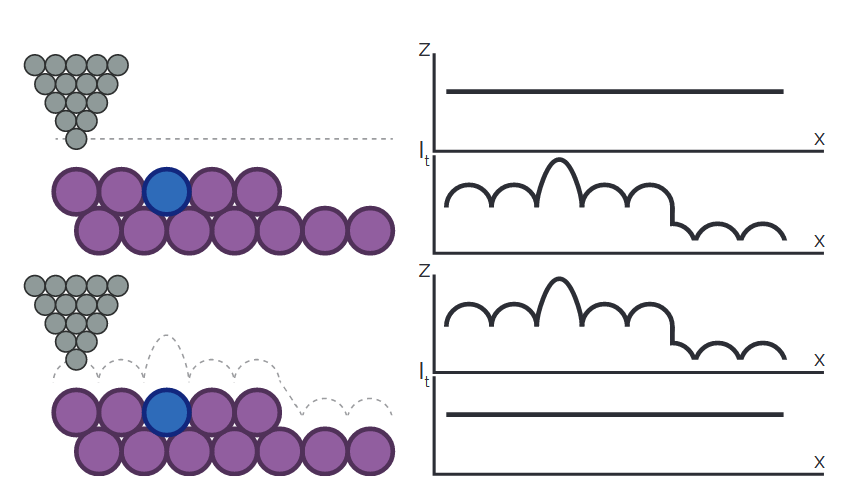
\includegraphics[width=0.8\textwidth]{topographic_modes.png}
	\caption{}
	\label{fig:topo_modes}
\end{figure}

The second mode of \ac{STM} operation is when we park the tip at a fixed position $\mathbf{r_0}$ within the tunneling region, and record the current while scanning the bias voltage. The result of such a measurement is an $I-V$ curve at $\mathbf{r} = \mathbf{r_0}$; by taking its derivative with respect to the voltage, we get the differential conductance, which is proportional to the sample's local electron density of state $\rho_s(\mathbf{r_0, E_F+eV})$. Another way to obtain the LDOS is through the use of a lockin-amplifier, which modulates the applied DC bias voltage $V_b$ by a sinusoidal AC voltage $V_{lockin}$.  $V_{lockin}$ normally has an amplitude of a few meV and a frequency $\omega$ ranging from a few hundred Hz to a few kHz. The extracted current response at $\omega$ is proportional to the differential conductance. The use of lock-in amplifier is particular useful in a noisy environment, since we can choose the lock-in frequency away from any noise peaks. This allows us to recover signal orders of magnitude smaller than the noise floor. However, despite being a powerful method, the use of lock-in has several limitations. The most significant is modulation broadening: the applied AC bias averages the signal over an energy window, which can smear out sharp spectral features and limit energy resolution. In addition, the lock-in assumes a fixed phase difference between the modulation and response; this means any phase lag, from either capacitance in the wiring of junction response time, can reduce the signal amplitude. Finally, the high sensitivity of lock-in detection often relies on long integration times, making measurements slower and less suited for systems with significant drift or low cryogenic holding time.

One can combine both the spatial and energy resolution of \ac{STM} by perform a spatial \ac{STS}, which is a way to collect local tunneling spectroscopy on many points on the material surface following a 2D grid. This give arise to a three-dimensional output data known as the grid map, which contains the spatially-variational electronic structure of the material. This makes \ac{STM} grid map spectroscopy a powerful mode in studying spatial features with characteristic \ac{LDOS}. At large scales, it has been widely used to probe emergent collective orders such as charge- and spin-density waves, which features periodic modulations of the local density of states. On intermediate scales, grid maps capture quasiparticle interference(QPI) patterns, enabling the reconstruction of electronic band dispersions in metal/semimetals, superconductors, and topological materials\cite{avrahamQuasiparticleInterferenceStudies2018}. Moving toward the nanoscale, they reveal spatial inhomogeneity in correlated systems, such as variations in the superconducting gap of high-Tc cuprates\cite{duanSingleparticleTunnelingSpectroscopy2021}\cite{boyerImagingTwoGaps2007} or the localized states in vortex cores of type-II superconductors\cite{panSTMStudiesElectronic2000}\cite{suderowImagingSuperconductingVortex2014}. Ultimately, at the atomic limit, grid maps excel at resolving the spatial variation of bound states attached to local defects — from donor or acceptor states in semiconductors\cite{mahieuDirectEvidenceShallow2005} to in-gap resonances near magnetic impurities\cite{schneiderMagnetismIngapStates2019}\cite{yangIngapQuasiparticleExcitations2013}\cite{chatzopoulosSpatiallyDispersingYuShibaRusinov2021}.

This study focus on revealing defect-specific information, and all three modes are used with different focus. Topographies are used to probe the spatial profiles and local distributions for different types of defects; these local distributions are used to calculate defect-specific populations. Point spectroscopies are taken to identify the defect-specific electronic structures. Grid maps are taken on regions with multiple defects to uncover their scattering patterns across different materials; they were then fed into the newly developed algorithm to resolve defect-specific \ac{QPI} features. 